\documentclass[a4paper]{article}
\usepackage{graphicx}
\usepackage{wrapfig}
\usepackage[export]{adjustbox}
\usepackage[margin=1in]{geometry}
\usepackage{fancyhdr}
\usepackage{tikz}
\usepackage[x11names]{xcolor}
\usepackage{listings}
\usepackage{chngcntr}
\usepackage{fmtcount}
\usepackage{romannum}
\usepackage{tcolorbox}
\tcbuselibrary{skins}
\usepackage{arabtex}
\usepackage{float}
\usepackage{utf8}
\setcode{utf8}
\usepackage{anyfontsize}
\usepackage{wrapfig}

% Alternative: For more control with fancyhdr
\pagestyle{fancy}
\fancyhf{}  % Clear all header/footer

% Header with caption and page number
%\fancyhead[L]{\textcolor{DodgerBlue4}{\textbf{AM Modulation Report}}}  

% Footer
\fancyfoot[R]{\thepage}  % Page number at right of footer
%\fancyfoot[L]{\textcolor{DeepSkyBlue4}{\textbf{Super-Heterodyne Receiver}}}  % Left footer caption

% Line thickness
\renewcommand{\headrulewidth}{0.2pt}
\renewcommand{\footrulewidth}{0.2pt}

% Add color to header rule
\makeatletter
\renewcommand{\headrule}{%
    \if@fancyplain\let\headrulewidth\plainheadrulewidth\fi
    \color{DodgerBlue4}\hrule\@height\headrulewidth\@width\headwidth\vskip-\headrulewidth
}
\renewcommand{\footrule}{%
    \if@fancyplain\let\footrulewidth\plainfootrulewidth\fi
    \color{DeepSkyBlue4}\hrule\@height\footrulewidth\@width\headwidth\vskip-\footrulewidth
}
\makeatother

\usepackage{listings}

%New colors defined below
\definecolor{titlecolor}{RGB}{0, 51, 102}
\definecolor{linecolor}{RGB}{200, 0, 0}
\definecolor{codegreen}{rgb}{0,0.6,0}
\definecolor{codegray}{rgb}{0.5,0.5,0.5}
\definecolor{codepurple}{rgb}{0.58,0,0.82}
\definecolor{backcolour}{rgb}{0.95,0.95,0.92}

%Code listing style named "mystyle"
\lstdefinestyle{mystyle}{
  backgroundcolor=\color{backcolour},
  commentstyle=\color{codegreen},
  keywordstyle=\color{magenta},
  numberstyle=\tiny\color{codegray},
  stringstyle=\color{codepurple},
  basicstyle=\ttfamily\footnotesize,
  breakatwhitespace=false,         
  breaklines=true,                 
  captionpos=b,                    
  keepspaces=true,                 
  numbers=left,                    
  numbersep=5pt,                  
  showspaces=false,                
  showstringspaces=false,
  showtabs=false,                  
  tabsize=2,
  language=MATLAB,
  morekeywords=[2]{audioread, sum, max, abs, length, size, plot, figure, subplot},
  sensitive=true
}

%"mystyle" code listing set
\lstset{style=mystyle}

\begin{document}
\pagenumbering{arabic} % Arabic/Indic page numbers
\begin{titlepage}
    % Header with logos
    \noindent
    \begin{minipage}[t]{0.3\textwidth}
    \includegraphics[width=3.5cm]{download.png}
\end{minipage}%
\hfill%
\begin{minipage}[t]{0.3\textwidth}
    \raggedleft
    \includegraphics[width=3.5cm]{Eng_Logo.png}
\end{minipage}
    
    % Title section
    \vspace*{2cm}
\begin{center}
    {\color{titlecolor}\fontsize{42}{48}\selectfont\bfseries AM Modulation}\\[0.5cm]
    \rule{0.8\textwidth}{2pt}\\[0.5cm]
    {\LARGE\textbf{Super-Heterodyne Receiver}}\\[1cm]
    
    % Subtitle
    {\Large A Technical Report on Design and Implementation}\\[1.5cm]
    
    % Decorative element
    
\begin{tikzpicture}
        \draw[linecolor, line width=1pt] (0,0) -- (10,0);
        \node[fill=white, inner sep=5pt] at (5,0) {\textbf{•••}};
    \end{tikzpicture}
\end{center}

% Author information - Centered
\vspace*{0.25cm}

    \begin{center}
    \textbf{\Large Supervised by:}\\[0.2cm]
    \large Dr. Ahmed Hesham\\[0.5cm]

    \textbf{\Large Presanted to:}\\[0.2cm]
    \large Eng. Mohamed Khalid\\[2cm]
    
    \fbox{\begin{tabular}{c|c}
    \large 91240727 & \large \RL{مروان محمد مبارك سليمان} \\
    \hline
    \large 12345678 & \large \RL{محمد احمد محمد محمد} 
\end{tabular}}\\[0.8cm]
    
\end{center}

% Footer
\end{titlepage}
\newpage
\tableofcontents
\newpage

% ==============================================================================
% SECTION I: Introduction
% ==============================================================================

\section*{\textcolor{DodgerBlue4}{\huge \Romannum{1}  Introduction}}
\vspace{0.5cm}
    \addcontentsline{toc}{section}{Introduction}
    \noindent\textcolor{DeepSkyBlue4}{\rule{\textwidth}{0.05pt}}
    
    \noindent This report documents the design and simulation of a complete AM (Amplitude Modulation) transceiver system implemented in MATLAB. The modulation scheme used is DSB-SC (Double Sideband Suppressed Carrier), and the receiver architecture is the classic super-heterodyne design. Two real audio signals are used as input messages, multiplexed over a shared channel using Frequency Division Multiplexing (FDM), and subsequently demodulated by the receiver chain.
    
    \vspace{\baselineskip}

    \noindent The simulation covers the following pipeline: audio preprocessing, DSB-SC modulation, FDM multiplexing, RF bandpass filtering, frequency down-conversion via a local oscillator and mixer, IF bandpass filtering, and final baseband detection with a low-pass filter. Spectrum plots are provided at each stage to verify correct operation. \vspace{1cm}
    
%% ==============================================================================
% SECTION II: BLOCK-BY-BLOCK DESIGN
% ==============================================================================  


\section*{\textcolor{DodgerBlue4}{\huge   \Romannum{2} Block-by-Block Design}}
    \vspace{0.5cm}
    \addcontentsline{toc}{section}{Block-by-Block Design}
    \noindent\textcolor{DeepSkyBlue4}{\rule{\textwidth}{0.05pt}}
%____________________________________________________________________________
%========================Signal Preprocessing==================
%____________________________________________________________________________
    
    \subsection*{\textcolor{DodgerBlue4}{\Large 2.1 Signal Preprocessing}}
    \addcontentsline{toc}{subsection}{Signal Preprocessing}
    
    
    Each .wav audio file is read using audioread(), which returns a stereo (2-channel) matrix and the sampling frequency Fs. The two channels are summed to produce a mono signal:
    
 %__________________________________CODE___________________________________________ 
\begin{lstlisting}[language = Matlab]
    [y_t, Fs] = audioread ('Short_BBCArabic2.wav');
    m_t = y_t(:,1) + y_t(:,2);                        
\end{lstlisting}
\vspace{\baselineskip}
%_____________________________________________________________________________ 
    
    \noindent Zero-padding is then applied to ensure both signals share the same length:
    
 %__________________________________CODE___________________________________________ 
\begin{lstlisting}[language = Matlab]
    max_length = max(length(m_t), length(a_t));
    m_t = [m_t; zeros(max_length - length(m_t), 1)];                        
\end{lstlisting}
\vspace{\baselineskip}
%_____________________________________________________________________________


    \noindent Finally, upsampling by a factor of 10 is applied using interp(). This is necessary because the carrier frequencies (100 kHz, 130 kHz) exceed Fs/2 = 22 kHz of the original audio, which would violate the Nyquist criterion. Upsampling raises the effective sampling rate to 441 kHz, satisfying Nyquist for all carrier frequencies used. 
%________________________________CODE_______________________________________
\begin{lstlisting}[language = Matlab]
    m_t = interp(m_t, 10);
    Fs  = Fs * 10;   % Fs is now 441000 Hz                     
\end{lstlisting}
\vspace{\baselineskip}
%_____________________________________________________________________________



%____________________________________________________________________________
%________________________DSB-SC Modulator___________________________________________
%____________________________________________________________________________

    \subsection*{\textcolor{DodgerBlue4}{\Large 2.2 DSB-SC Modulator \& FDM Multiplexing}} \addcontentsline{toc}{subsection}{DSB-SC Modulator \& FDM Multiplexing}
    
    \noindent Each message signal is modulated using DSB-SC: the message is multiplied element-wise by a cosine carrier at the assigned frequency. DSB-SC produces no carrier component in the transmitted spectrum only the two sidebands around carrier frequency.
    The mathematical operation is:
    
    %___________________________CODE__________________________________
\begin{lstlisting}[language = Matlab]
    modulated_signal_1 = m_t ' .* cos (2* pi * Fc_1 * t ) ; % DSB - SC : BBC @ 100 kHz
    modulated_signal_2 = a_t ' .* cos (2* pi * Fc_2 * t ) ; % DSB - SC : FM @ 130 kHz
    Tx_signal = modulated_signal_1 + modulated_signal_2 ;   % DSB - SC : FM + BBC 
\end{lstlisting}
\vspace{\baselineskip}
%________________________________________________________________________


%+++++++++++++++++++++++++++Modulator diagram figure+++++++++++++++++++++++++
 \begin{figure}[h]
        \centering
        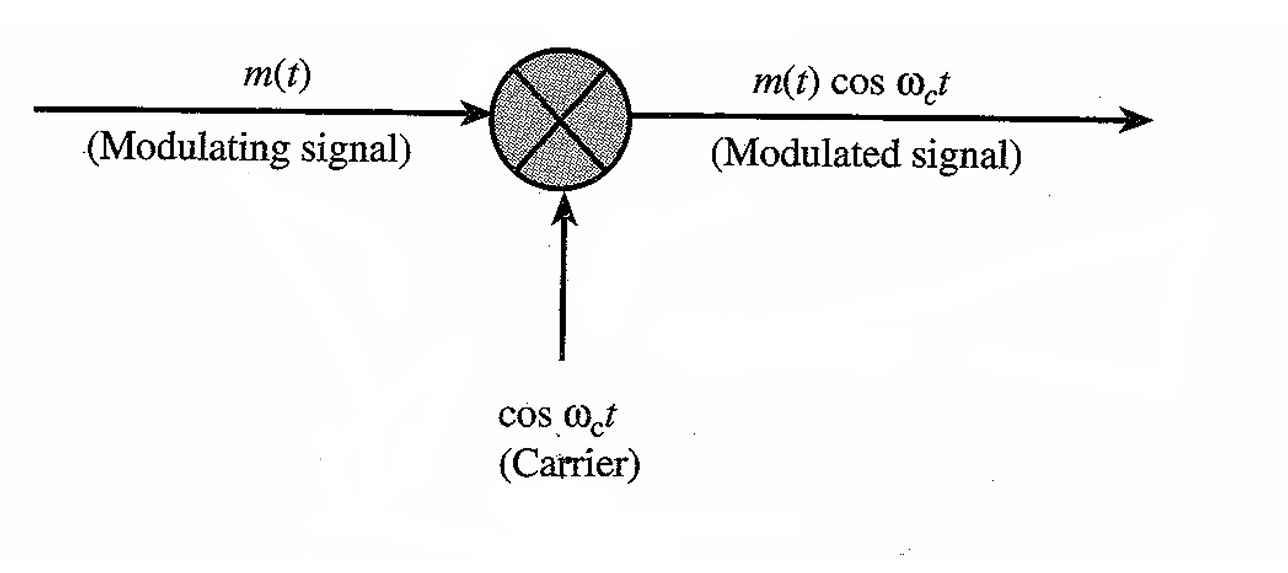
\includegraphics[width=0.6\textwidth]{Modulator.png}
        \caption{\small{Transimitter (Coherent Modulator Block)}}
        \label{fig:plot2}
        \end{figure}
%_____________________________________________________________________________

        
%____________________________________________________________________________
%___________________________RF Stage - Band-pass Filter_________________________
%____________________________________________________________________________

\subsection*{\textcolor{DodgerBlue4}{\Large 2.3 RF Stage — Band-Pass Filter}}
\addcontentsline{toc}{subsection}{RF Stage — Band-Pass Filter}
\noindent The RF stage is implemented as band-pass filter centered at the desired station carrier frequency. and each signal bandwidth is roughly estimated from frequency spectrum plot.  Its role is to select only one station from the FDM composite and reject all others, including potential image-frequency interference.

%___________________________CODE__________________________________
\begin{lstlisting}[language = Matlab]
    fpass_RF            = [Fc_desired - Bw_desired Fc_desired + Bw_desired];  
    modulated_signal_RF = bandpass(Tx_signal, fpass_RF, Fs);  
\end{lstlisting}
\vspace{\baselineskip}
%____________________________________________________________________


%____________________________________________________________________________
%__________________________________Local Oscillator__________________________
%____________________________________________________________________________

\subsection*{\textcolor{DodgerBlue4}{\Large 2.4 Local Oscillator \& Mixer}}
\addcontentsline{toc}{subsection}{Local Oscillator \& Mixer}
\noindent The local oscillator generates a cosine at frequency $F_{lo} = F_c + F_{IF} = 115$ kHz. The mixer multiplies the RF-filtered signal by this oscillator, which frequency-shifts the desired station from 100 kHz down to the fixed intermediate frequency of 15 kHz:
%___________________________CODE__________________________________
\begin{lstlisting}[language = Matlab]
    F_lo   = Fc_desired + F_IF;          
    S_mixed = modulated_signal_RF .* cos(2*pi*F_osc*t);  
\end{lstlisting}
\vspace{\baselineskip}
%____________________________________________________________________


After mixing, the spectrum contains two components: the desired signal at $F_{IF} = 15$ kHz and an unwanted high-frequency image at $2×F_{c} + F_{IF} = 215$ kHz. The IF stage removes this image.


%____________________________________________________________________________
%____________________________IF stage - Band Pass Filter_____________________
%____________________________________________________________________________


\subsection*{\textcolor{DodgerBlue4}{\Large 2.5 IF Stage — Band-Pass Filter}}
\addcontentsline{toc}{subsection}{IF Stage — Band-Pass Filter}
\noindent IF stage is a second BPF centered at $F_{IF} = 15$ kHz. It passes only the down-converted desired signal and removes the high-frequency image produced by the mixer as well as any residual interference:


%___________________________CODE__________________________________
\begin{lstlisting}[language = Matlab]
    fpass_IF = [F_IF - Bw_desired, F_IF + Bw_desired];
    modulated_signal_IF = bandpass(S_mixed, fpass_IF, Fs);

\end{lstlisting}
\vspace{\baselineskip}
%_____________________________________________________________________


%____________________________________________________________________________
%______________________________Baseband Detection____________________________
%____________________________________________________________________________

\subsection*{\textcolor{DodgerBlue4}{\Large 2.6 Baseband Detection}}
\addcontentsline{toc}{subsection}{Baseband Detection}
\noindent The baseband detector performs the final demodulation in two steps. First, the IF signal is multiplied by a cosine at $F_{IF} = 15$ kHz. This shifts the signal spectrum from 15 kHz back to 0 Hz (baseband) but also creates a high-frequency image at $2F_{IF} = 30$ kHz. Then a low-pass filter designed with fdesign.lowpass then removes the 30 kHz image and leaves only the recovered audio signal in the baseband:

%___________________________CODE__________________________________
\begin{lstlisting}[language = Matlab]
    S_BB = S_IF .* cos(2*pi*F_IF*t);
    d_lpf       = fdesign.lowpass('N,F3dB', 6, Bw_desired/(Fs/2));
    hLPF        = design(d_lpf, 'butter');
    Rx_signal   = filter(hLPF, S_BB);
\end{lstlisting}
%______________________________________________________________________

The specification string \textbf{'N,F3dB'} tells \textbf{fdesign.lowpass} that the filter is defined by its order (N=6) and its 3 dB cutoff frequency, which is normalized to the range [0,1] by dividing by $F_s/2$.
\vspace{1.5cm}

%++++++++++++++++++++++++Receiver-block-diagram Figure++++++++++++++
\begin{figure}[h]
        \centering
        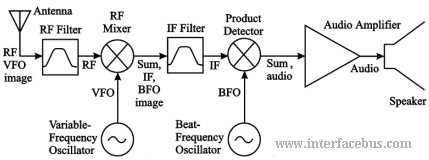
\includegraphics[width=0.6\textwidth]{receiver-block-diagram.jpg}
        \caption{\small{Super heterodyne receiver block }}
        \label{fig:plot2}
        \end{figure}
%______________________________________________________________________________


% ==============================================================================
% SECTION IV: Discussion
% ==============================================================================
\section*{\textcolor{DodgerBlue4}{\huge   \Romannum{3} Discussion}}
    \vspace{0.5cm}
    \addcontentsline{toc}{section}{Discussion}
    \noindent\textcolor{DeepSkyBlue4}{\rule{\textwidth}{0.05pt}}
%_____________________________________________________________________________

    
%_____________________________________________________________________________
%__ __________Role of RF , IF , and Baseband_____________________________________
%____________________________________________________________________________
    
    \subsection*{\textcolor{DodgerBlue4}{\Large \romannum{1}. Role of RF, IF, and Baseband Stages}}\addcontentsline{toc}{subsection}{Role of RF, IF, and Baseband Stages}

    
    \noindent The RF stage is a tunable band-pass filter at the antenna. Its primary role is image-frequency rejection: it selects only the desired station carrier and suppresses all other stations and interference before the signal reaches the mixer.\\
   \noindent The IF stage is a fixed band-pass filter at the intermediate frequency (15 kHz in this simulation). Because the IF frequency is always constant regardless of which station is selected, the IF filter can be designed once with very tight, optimized characteristics. This is the key advantage of the super-heterodyne architecture: selectivity and sensitivity are achieved at a fixed, low IF rather than at the variable RF carrier.\\
    The baseband detector performs the final down-conversion from $F_{IF}$ to 0 Hz and applies a low-pass filter to recover the original audio message. Without this stage the signal would remain modulated at the intermediate frequency and would not be audible.\\
    \vspace{0.4cm}
    %____________________________________________________________________________
    
    \noindent \textbf{Why do we need the IF stage?} Designing a sharp, stable BPF at RF frequencies (100 kHz, 130 kHz) is difficult because small component tolerances cause large frequency errors at high frequencies. By first converting the signal to a lower, fixed IF, the demanding filtering work is done at 15 kHz where filters are far easier to build and keep stable.

    
%____________________________________________________________________________
%_____Spectrum at Each Stage_________________________________________________
%____________________________________________________________________________


    \subsection*{\textcolor{DodgerBlue4}{\Large \romannum{2}. Spectrum at Each Stage (Demodulating Station 1)}}\addcontentsline{toc}{subsection}{Spectrum at Each Stage}
    \noindent The following describes the expected spectral content observed at the output of each stage when demodulating Station 1 (BBC Arabic at $F_c = 100$ kHz):


    \begin{itemize}
        \item \large {\textbf{After RF BPF}}
        \normalsize{The FDM composite spectrum contains two pairs of sidebands at ±100 kHz and ±130 kHz. After the RF BPF (passband 92–108 kHz), only the sideband pair at ±100 kHz remains. The 130 kHz station is fully suppressed.}  
    
    \begin{figure}[h]
        \centering
        \includegraphics[width=0.8\textwidth]{rf_stage_output.png}
        \caption{\small{Modulated Signal in RF spectrum}}
        \label{fig:plot1}
    \end{figure}
    \end{itemize}
\newpage



    \begin{itemize}
        \item \large {\textbf{After IF BPF}}
        \normalsize {After mixing with the 115 kHz oscillator, the 100 kHz signal shifts to 15 kHz. A high-frequency image also appears at approximately 215 kHz. The IF BPF (passband 7–23 kHz) retains only the 15 kHz component and removes the image.}   
        
        \begin{figure}[h]
        \centering
        \includegraphics[width=0.8\textwidth]{IF_Stage_Output.png}
        \caption{\small{Modulated Signal in IF spectrum}}
        \label{fig:plot2}
        \end{figure}
    \end{itemize}


    
    \begin{itemize}
        \item \large {\textbf{After Baseband Detection}}
        \normalsize {Multiplying by $cos(2\pi15000t)$ shifts the IF signal to baseband (0 Hz). The LPF removes the 30 kHz image, leaving a clean spectrum centered at 0 Hz with bandwidth equal to the original audio signal (approximately 8 kHz for speech).}
        
        \begin{figure}[H]
        \centering
        \includegraphics[width=0.8\textwidth]{BaseBand_output.png}
        \caption{\small{Received Signal spectrum}}
        \label{fig:plot3}
        \end{figure}
        
    \end{itemize}

    
%____________________________________________________________________________
%___ Effect of Removing RF BPF_____________________________________________
%____________________________________________________________________________


    \subsection*{\textcolor{DodgerBlue4}{\Large \romannum{3}. Effect of Removing the RF BPF}}
    \addcontentsline{toc}{subsection}{Effect of Removing the RF BPF}
\noindent When the RF BPF is removed both stations land at the same IF frequency. The IF BPF cannot distinguish 
between them because they now fully overlap in the spectrum. The result at baseband 
is a superposition of both audio streams, making the recovered audio heard simultaneously and interfere with each other.\\[3pt]
This clearly demonstrates the critical role of the RF stage: it performs 
image-frequency rejection, ensuring that only the desired station reaches the mixer.


%_____________________________________________________________________________
% ── Figure 1: RF output without BPF ─────────────────────────────────────────
%_____________________________________________________________________________

\vspace{8pt}
\noindent\textbf{RF Stage (No BPF Applied)}\\[4pt]
\noindent Without the RF band-pass filter, the full FDM composite signal containing 
both stations at 100\,kHz and 130\,kHz passes directly into the mixer. As seen in 
Figure~\ref{fig:plot4}, both sidebands are clearly present with equal strength — 
neither station has been rejected.

\begin{figure}[h]
    \centering
    \includegraphics[width=0.8\textwidth]{RF_no_BPF.png}
    \caption{\small{RF stage input spectrum without BPF }}
    \label{fig:plot4}
\end{figure}


%_____________________________________________________________________________
% ── Figure 2: IF output without RF BPF ──────────────────────────────────────
%_____________________________________________________________________________


\vspace{4pt}
\noindent\textbf{ IF Stage Output }\\[4pt]
\noindent After mixing with the local oscillator at $F_c + F_{IF}$, both stations 
are down-converted and land at the same intermediate frequency of 15\,kHz. 
Figure~\ref{fig:plot5} shows that the two signals fully overlap at the IF, making 
it impossible for the IF BPF to separate them. The filter passes both signals 
together, as they are indistinguishable at this stage.
\vspace{4pt}

\begin{figure}[H]
    \centering
    \includegraphics[width=0.85\textwidth]{IF_no_RF_BPF.png}
    \caption{\small{IF stage output spectrum without RF BPF }}
    \label{fig:plot5}
\end{figure}


%___________________________________________________________________________
% ── Figure 3: Recovered baseband without RF BPF ──────────────────────────────
%____________________________________________________________________________


\vspace{4pt}
\noindent\textbf{Recovered Baseband Signal }\\[4pt]
\noindent At the baseband detection output, Figure~\ref{fig:plot6} shows a 
corrupted spectrum where the energy of both audio stations is superimposed across 
the entire baseband band. Unlike the clean single-lobe spectrum obtained with the 
RF BPF active, this spectrum contains the mixed content of both stations. When 
played back using \texttt{sound()}, the output is unintelligible — both broadcasts 
are audible simultaneously with heavy mutual interference.

\begin{figure}[h]
    \centering
    \includegraphics[width=0.85\textwidth]{BaseBand_no_RF_BPF.png}
    \caption{\small{Recovered baseband spectrum without RF BPF}}
    \label{fig:plot6}
\end{figure}
\vspace{6pt}
\noindent\textbf{Conclusion of this experiment:} The RF band-pass filter is not 
optional. Without it, the super-heterodyne receiver loses its ability to tune to 
a single station. Any signal whose frequency satisfies $|F - F_{lo}| = F_{IF}$ 
will alias directly onto the desired channel at the IF stage, an effect known as 
\textit{image-frequency interference}. The RF BPF is the only stage that can 
reject this image before it corrupts the received signal.\\[8pt]


%_____________________________________________________________________________
%_____________________________EFFECT OF oscillator offset _______________________
%_____________________________________________________________________________


\subsection*{\textcolor{DodgerBlue4}{\Large \romannum{4}. Effect of Oscillator Frequency Offset}}
\addcontentsline{toc}{subsection}{Effect of Oscillator Frequency Offset}

\vspace{6pt}

% ── Small Offset ────────────────────────────────────────────────────────────
\noindent{\large\textbf{Small Offset (0.1 kHz)}}

\vspace{4pt}
\noindent In this case, the signal shifts from 15\,kHz to 15.1\,kHz.

\vspace{6pt}
\noindent\begin{tabular}{@{} p{2.8cm} p{10.5cm} @{}}
    \textbf{Spectrum} & All frequency components move to the right by 100\,Hz. \\[8pt]
    \textbf{Audio}    & The speech is still clear, but the pitch is slightly higher. 
                        The voice sounds a little different (change in timbre), but 
                        you can still understand everything easily. \\
\end{tabular}

\vspace{14pt}
\hrule height 0.3pt
\vspace{14pt}

% ── Large Offset ────────────────────────────────────────────────────────────
\noindent{\large\textbf{Large Offset (1 kHz)}}

\vspace{4pt}
\noindent Here, the signal shifts much further to 16\,kHz.

\vspace{6pt}
\noindent\begin{tabular}{@{} p{2.8cm} p{10.5cm} @{}}
    \textbf{Spectrum} & There is a large 1\,kHz shift to the right. Because of 
                        this, the Low-Pass Filter (LPF) may cut off the higher 
                        parts of the signal. \\[8pt]
    \textbf{Audio}    & The voice sounds very unnatural and robotic. It is much 
                        harder to understand the speech because the frequencies 
                        are pushed too far from their original place. \\
\end{tabular}

\vspace{14pt}
\hrule height 0.3pt
\vspace{14pt}

% ── Conclusion ───────────────────────────────────────────────────────────────
\noindent{\large\textbf{Conclusion}}

\vspace{4pt}
\noindent This experiment proves that the Local Oscillator must be very stable. 
If the frequency is even slightly wrong, the output audio changes. In real-world 
receivers, we use a Phase-Locked Loop (PLL) like Costas Loop to ``lock'' the 
frequency and make sure the local oscillator stays exactly on the correct frequency.\\



\section*{\textcolor{DodgerBlue4}{\huge \Romannum{4}  MATLAB Source Code}}
\vspace{0.5cm}
    \addcontentsline{toc}{section}{MATLAB Source Code}
    \noindent\textcolor{DeepSkyBlue4}{\rule{\textwidth}{0.05pt}}

    
    \begin{lstlisting}[language = Matlab]
% Amplitude Modulation - Super Heterodyne Receiver
% Author : Marwan Mobarak
% Date   : 4/3/2026

%% ====================== File Processing ================================
[y_t, Fs1] = audioread("Short_BBCArabic2.wav");
m_t = y_t(:,1) + y_t(:,2);                     % Stereo to Mono

[z_t, Fs2] = audioread("Short_FM9090.wav");
a_t = z_t(:,1) + z_t(:,2);                     % Stereo to Mono

Fs = max(Fs1, Fs2);                             % Use higher sampling rate

clear y_t z_t Fs1 Fs2;

%% ====================== Zero Padding ===================================
max_length = max(length(m_t), length(a_t));
m_t = [m_t; zeros(max_length - length(m_t), 1)];  
a_t = [a_t; zeros(max_length - length(a_t), 1)];  

%% ====================== Upsampling =====================================
upsample_factor = 10;
m_t        = interp(m_t, upsample_factor);
a_t        = interp(a_t, upsample_factor);
Fs         = Fs * upsample_factor;              % 441000 Hz
Ts         = 1/Fs;
max_length = length(m_t);

%% ======================== AM Modulator (DSB-SC) ========================
Fc_1 = 100000;                                  % Station 1: 100 kHz
Fc_2 = 130000;                                  % Station 2: 130 kHz
Bw_1 = 8000;                                    % Baseband BW station 1
Bw_2 = 8000;                                    % Baseband BW station 2

t    = (0 : max_length-1) * Ts;                 % Time vector

modulated_signal_1 = m_t' .* cos(2*pi*Fc_1*t);               % DSB-SC: BBC @ 100 kHz
modulated_signal_2 = a_t' .* cos(2*pi*Fc_2*t);               % DSB-SC: FM  @ 130 kHz
Tx_signal          = modulated_signal_1 + modulated_signal_2;                             % FDM composite signal

%% ======================== RF Stage =====================================
Fc_desired           = Fc_1;                             % Tune to Station 1
Bw_desired           = Bw_1;

 fpass_RF            = [Fc_desired - Bw_desired Fc_desired + Bw_desired];        % [92000, 108000] Hz
 modulated_signal_RF = bandpass(Tx_signal, fpass_RF, Fs);     

%% ======================== Mixer ========================================
F_IF        = 15000;                            % IF frequency: 15 kHz
Offset      = 100 ;
F_lo        = Fc_desired + F_IF + Offset ;       % Oscillator: 115 kHz
S_mixed     = modulated_signal_RF .* cos(2*pi*F_lo*t);         % Shift 100kHz to 15kHz

%% ======================== IF Stage =====================================
fpass_IF            = [F_IF - Bw_desired, ...
                       F_IF + Bw_desired];              % [7000, 23000] Hz
modulated_signal_IF = bandpass(S_mixed, fpass_IF, Fs);

%% ======================== Baseband Detection ===========================
S_BB        = modulated_signal_IF .* cos(2*pi*F_IF*t);        % Shift 15kHz to 0Hz

d_lpf       = fdesign.lowpass(    ...
    'N,F3dB'          ,           ...           % Spec: order + 3dB cutoff
    6                 ,           ...           % Filter order
    Bw_desired/(Fs/2)             );            % Normalized cutoff

hLPF        = design(d_lpf, 'butter');          % Butterworth LPF
Rx_signal = filter(hLPF, S_BB);              % Recovered message

%% ======================== Listen & Plot ================================
% Downsample to playable rate before sound()
N1 = length(m_t);
f1 = (0:N1-1) * (Fs/N1);
N2 = length(a_t);
f2 = (0:N2-1) * (Fs/N2);
Fs_play     = 44100;                            % Standard audio rate
m_play      = Rx_signal(1:upsample_factor:end); % Decimate by 10
sound(m_play, Fs_play);                         % Play recovered audio

% Plot recovered signal spectrum
figure('Name','Recovered Signal','NumberTitle','off');
N   = length(Rx_signal);
f   = (-N/2 : N/2-1) * (Fs/N);
plot(f, abs(fftshift(fft(Rx_signal)))/N, 'g', 'LineWidth', 1.2);
xlabel('Frequency (Hz)'); ylabel('Magnitude');
title('Recovered Baseband Signal - BBC Arabic');
xlim([-15000 15000]); grid on;

%% --- 1. RF Stage Output ------------------------------------------------
figure('Name','RF Stage Output','NumberTitle','off');

N_rf  = length(modulated_signal_RF);
f_rf  = (-N_rf/2 : N_rf/2-1) * (Fs / N_rf);   % Two-sided frequency axis (Hz)
Y_rf  = abs(fftshift(fft(modulated_signal_RF))) / N_rf;        % Normalized magnitude spectrum

plot(f_rf, Y_rf, 'b', 'LineWidth', 1.4);
xlabel('Frequency (Hz)');
ylabel('Magnitude');
title('RF Stage Output Spectrum');
xlim([-200000 200000]);
ylim([0 max(Y_rf)*1.2]);
grid on;

% Mark the selected carrier on both sides
xline( Fc_desired, 'r--', sprintf('+Fc = %d kHz', Fc_desired/1000), ...
       'LabelVerticalAlignment', 'bottom', 'LineWidth', 1.5);
xline(-Fc_desired, 'r--', sprintf('-Fc = %d kHz', Fc_desired/1000), ...
       'LabelVerticalAlignment', 'bottom', 'LineWidth', 1.5);

legend('RF Output', 'Selected carrier');

%% --- 2. IF Stage Output ------------------------------------------------
figure('Name','IF Stage Output','NumberTitle','off');

N_if  = length(modulated_signal_IF);
f_if  = (-N_if/2 : N_if/2-1) * (Fs / N_if);   % Two-sided frequency axis (Hz)
Y_if  = abs(fftshift(fft(modulated_signal_IF))) / N_if;        % Normalized magnitude spectrum

plot(f_if, Y_if, 'r', 'LineWidth', 1.4);
xlabel('Frequency (Hz)');
ylabel('Magnitude');
title('IF Stage Output Spectrum');
xlim([-50000 50000]);
ylim([0 max(Y_if)*1.2]);
grid on;

% Mark the IF center frequency on both sides
xline( F_IF, 'b--', sprintf('+F_{IF} = %d kHz', F_IF/1000), ...
       'LabelVerticalAlignment', 'bottom', 'LineWidth', 1.5);
xline(-F_IF, 'b--', sprintf('-F_{IF} = %d kHz', F_IF/1000), ...
       'LabelVerticalAlignment', 'bottom', 'LineWidth', 1.5);

legend('IF Output', 'IF center frequency');

%% --- 3. Baseband Stage Output ------------------------------------------
figure('Name','Baseband Detection Output','NumberTitle','off');

N_bb  = length(Rx_signal);
f_bb  = (-N_bb/2 : N_bb/2-1) * (Fs / N_bb);   % Two-sided frequency axis (Hz)
Y_bb  = abs(fftshift(fft(Rx_signal))) / N_bb; % Normalized magnitude spectrum

plot(f_bb, Y_bb, 'g', 'LineWidth', 1.4);
xlabel('Frequency (Hz)');
ylabel('Magnitude');
title('Baseband Detection Output Spectrum (Recovered Message)');
xlim([-15000 15000]);
ylim([0 max(Y_bb)*1.2]);
grid on;

% Mark the bandwidth boundary
xline( Bw_desired, 'k--', sprintf('+Bw = %d kHz', Bw_desired/1000), ...
       'LabelVerticalAlignment', 'bottom', 'LineWidth', 1.5);
xline(-Bw_desired, 'k--', sprintf('-Bw = %d kHz', Bw_desired/1000), ...
       'LabelVerticalAlignment', 'bottom', 'LineWidth', 1.5);

legend('Recovered baseband', 'Bandwidth limit');
\end{lstlisting}
    
\end{document}
